\documentclass{beamer}
\usepackage[utf8]{inputenc}

\usetheme{Madrid}
\usecolortheme{default}
\usepackage{amsmath,amssymb,amsfonts,amsthm}
\usepackage{txfonts}
\usepackage{tkz-euclide}
\usepackage{listings}
\usepackage{adjustbox}
\usepackage{array}
\usepackage{tabularx}
\usepackage{gvv}
\usepackage{lmodern}
\usepackage{circuitikz}
\usepackage{tikz}
\usepackage{graphicx}
\usepackage{mathtools}
\setbeamertemplate{page number in head/foot}[totalframenumber]

\usepackage{tcolorbox}
\tcbuselibrary{minted,breakable,xparse,skins}



\definecolor{bg}{gray}{0.95}
\DeclareTCBListing{mintedbox}{O{}m!O{}}{%
  breakable=true,
  listing engine=minted,
  listing only,
  minted language=#2,
  minted style=default,
  minted options={%
    linenos,
    gobble=0,
    breaklines=true,
    breakafter=,,
    fontsize=\small,
    numbersep=8pt,
    #1},
  boxsep=0pt,
  left skip=0pt,
  right skip=0pt,
  left=25pt,
  right=0pt,
  top=3pt,
  bottom=3pt,
  arc=5pt,
  leftrule=0pt,
  rightrule=0pt,
  bottomrule=2pt,
  toprule=2pt,
  colback=bg,
  colframe=orange!70,
  enhanced,
  overlay={%
    \begin{tcbclipinterior}
    \fill[orange!20!white] (frame.south west) rectangle ([xshift=20pt]frame.north west);
    \end{tcbclipinterior}},
  #3,
}
\lstset{
    language=C,
    basicstyle=\ttfamily\small,
    keywordstyle=\color{blue},
    stringstyle=\color{orange},
    commentstyle=\color{green!60!black},
    numbers=left,
    numberstyle=\tiny\color{gray},
    breaklines=true,
    showstringspaces=false,
}

\title 
{1.6.12}
\date{August 26, 2025}


\author 
{Vivek K Kumar - EE25BTECH11062}



\begin{document}


\frame{\titlepage}
\begin{frame}{Question}
Show that point \myvec{-4 \\ 2} lies on the line segment joining the points \textbf{A} \myvec{-4 \\ 6} and \textbf{B} \myvec{-4 \\ -6}.
\end{frame}



\begin{frame}{Variables used}
\begin{table}[H]    
  \centering
  

  \caption{Variables Used}
  \label{tab:1.6.12}
\end{table}

\end{frame}

\begin{frame}{Solution}

The Collinearity matrix is given by\\
\begin{align}
\myvec{
   \vec{B}-\vec{A} & \vec{C}-\vec{A}
 }^T = \myvec{
   0 & -12 \\
   0 & -4
   }\\
 \xleftrightarrow[]{R_2 \rightarrow {R_2-\frac{1}{3}R_1}}
 \myvec{
   0 & -12
   \\
   0 & 0
   }
\end{align}
Since the rank of the Collinearity matrix is $1$, the points are collinear

\end{frame}

\begin{frame}[fragile]
    \frametitle{Python - Importing libraries and checking system}
    \begin{lstlisting}
import sys
import numpy as np
import numpy.linalg as LA
import matplotlib.pyplot as plt
import matplotlib.image as mpimg

from libs.line.funcs import *
from libs.triangle.funcs import *
from libs.conics.funcs import circ_gen

import subprocess
import shlex

print('Using termux?(y/n)')
y = input()
\end{lstlisting}
\end{frame}

\begin{frame}[fragile]
    \frametitle{Python - Checking collinearity}
    \begin{lstlisting}
A = np.array([-4, 6]).reshape(-1, 1)
B = np.array([-4, -6]).reshape(-1, 1)
C = np.array([-4, 2]).reshape(-1, 1)

collinearity_matrix = np.column_stack([B-A, C-A]).T
rank = LA.matrix_rank(collinearity_matrix)

if(rank == 1):
    print('The given points are collinear as the rank of the collinearity matrix is 1')
else:
    print('The given points are not collinear as the rank of the collinearity matrix is not 1')
\end{lstlisting}
\end{frame}

\begin{frame}[fragile]
    \frametitle{Python - Generating points and plotting}
    \begin{lstlisting}
p_AB = line_gen(A, B)
p_AC = line_gen(A, C)
p_CB = line_gen(C, B)

plt.plot(p_AB[0, :], p_AB[1, :], label = 'Line through AB')
plt.plot(p_AC[0, :], p_AC[1, :], label = 'Line through AC')
plt.plot(p_CB[0, :], p_CB[1, :], label = 'Line through CB')
\end{lstlisting}
\end{frame}

\begin{frame}[fragile]
    \frametitle{Python - Labelling points}
    \begin{lstlisting}
line_coords = np.block([[A,B,C]])
plt.scatter(line_coords[0,:], line_coords[1,:])
vert_labels = ['A','B','C']
for i, txt in enumerate(vert_labels):
    plt.annotate(txt, 
                 (line_coords[0,i], line_coords[1,i]),
                 textcoords="offset points", 
                 xytext=(0,10),
                 ha='center')

plt.xlabel('$x$')
plt.ylabel('$y$')
plt.legend(loc='best')
plt.grid() 
plt.axis('equal')
    \end{lstlisting}
\end{frame}

\begin{frame}[fragile]
    \frametitle{Python - Saving figure and opening it}
    \begin{lstlisting}
        plt.savefig('../figs/fig.png')
        print('Saved figure to ../figs/fig.png')
        
        if(y == 'y'):
            subprocess.run(shlex.split('termux-open ../figs/fig.png'))
        else:
            subprocess.run(["open",  "../figs/fig.png"])
    \end{lstlisting}
\end{frame}


\begin{frame}{Plot-Using only Python}
    \centering
    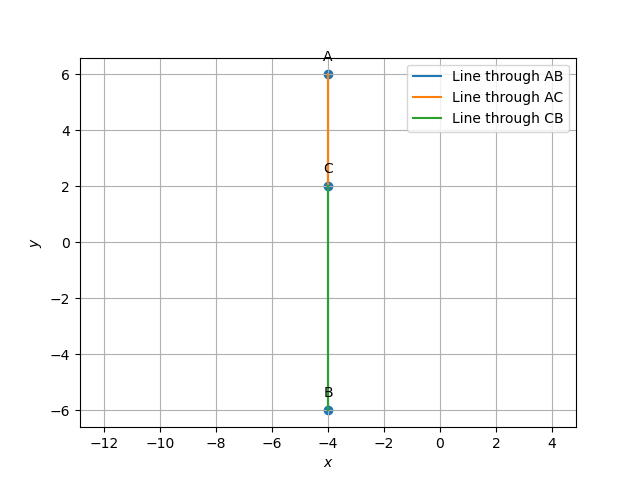
\includegraphics[width=\columnwidth, height=0.8\textheight, keepaspectratio]{../figs/fig.png}     
\end{frame}

\begin{frame}[fragile]
    \frametitle{C Code (0) - Importing libraries}

    \begin{lstlisting}
#include <stdio.h>
#include <stdlib.h>
#include <string.h>
#include <math.h>
#include <sys/socket.h>
#include <netinet/in.h>
#include <unistd.h>
#include "libs/matfun.h"
#include "libs/geofun.h"
    \end{lstlisting}
\end{frame}
\begin{frame}[fragile]
    \frametitle{C Code (1) - Function to Generate Points on a Line}

    \begin{lstlisting}

void point_gen(FILE *p_file, double **A, double **B, int rows, int cols, int npts){
    for(int i = 0; i <= npts; i++){
     double **output = Matadd(A, Matscale(Matsub(B, A, rows, cols), rows, cols, (double)i/npts), rows, cols);
     fprintf(p_file, "%lf, %lf\n", output[0][0], output[1][0]);
     freeMat(output, rows);
    } 
}

    \end{lstlisting}
\end{frame}


\begin{frame}[fragile]
    \frametitle{C Code (2) - Function to write points b/w given points to a file}

    \begin{lstlisting}

void write_points(double x1, double y1, double x2, double y2, int npts){
    int m = 2;
    int n = 1;

    double **A = createMat(m, n);
    double **B = createMat(m, n);

    A[0][0] = x1;
    A[1][0] = y1;

    B[0][0] = x2;
    B[1][0] = y2;
    \end{lstlisting}
\end{frame}
\begin{frame}[fragile]
    \frametitle{C Code (2) - Function to write points b/w given points to a file}

    \begin{lstlisting}
    FILE *p_file;
    p_file = fopen("plot.dat", "w");
    if(p_file == NULL){
        printf("Error opening data file\n");
    }

    point_gen(p_file, A, B, m, n, npts);

    freeMat(A, m);
    freeMat(B, m);

    fclose(p_file);
}


    \end{lstlisting}
\end{frame}

\begin{frame}[fragile]
    \frametitle{C Code (3) - Checking if points are collinear}

    \begin{lstlisting}

int check_collinearity(double x1, double y1, double x2, double y2, double x3, double y3){
     int m = 2;
     int n = 1;

     double **A = createMat(m, n);
     double **B = createMat(m, n);
     double **C = createMat(m, n);

     A[0][0] = x1;
     A[1][0] = y1;

     B[0][0] = x2;
     B[1][0] = y2;

     C[0][0] = x3;
     C[1][0] = y3;

    \end{lstlisting}
\end{frame}


\begin{frame}[fragile]
    \frametitle{C Code (3) - Checking if points are collinear}

    \begin{lstlisting}
     double **collinearity_matrix = transposeMat(Mathstack(Matsub(B, A, m, n), Matsub(C, A, m, n), m, n , n), m, n*2);
     double **eigvals = Mateigval(collinearity_matrix);


     int rank = 0;
     for (int i = 0; i < 2; i++) {
        if (fabs(eigvals[i][0]) > 1e-9) rank++;
     }

     freeMat(A, m);
     freeMat(B, m);
     freeMat(C, m);
     freeMat(collinearity_matrix, m);
     freeMat(eigvals, m);


\end{lstlisting}
\end{frame}

\begin{frame}[fragile]
    \frametitle{C Code (3) - Checking if points are collinear}

    \begin{lstlisting}
     if(rank == 1){
         return 1;
     }
     else{
         return 0;
     }
}
    \end{lstlisting}
\end{frame}

\begin{frame}[fragile]
    \frametitle{Python Code (0) - Importing libraries and checking system}
    \begin{lstlisting}
import numpy as np
import matplotlib.pyplot as plt
import ctypes
import os
import sys
import subprocess

print('Using termux? (y/n)')
termux = input()
\end{lstlisting}
\end{frame}

\begin{frame}[fragile]
    \frametitle{Python Code (1) - Using Shared Object}
    \begin{lstlisting}
lib_path = os.path.join(os.path.dirname(__file__), 'plot.so')
my_lib = ctypes.CDLL(lib_path)

my_lib.write_points.argtypes = [ctypes.c_double, ctypes.c_double, ctypes.c_double, ctypes.c_double, ctypes.c_int]
my_lib.write_points.restype = None
my_lib.write_points(-4, 6, -4, -6, 20000)

my_lib.check_collinearity.argtypes = [ctypes.c_double, ctypes.c_double, ctypes.c_double, ctypes.c_double, ctypes.c_double, ctypes.c_double]
my_lib.check_collinearity.restype = ctypes.c_int
collinearity = my_lib.check_collinearity(-4, 6, -4, -6, -4, 2)
\end{lstlisting}
\end{frame}

\begin{frame}[fragile]
    \frametitle{Python Code (2) - Handling collinearity}
    \begin{lstlisting}
if (collinearity == 1):
    print('The given points are collinear and the rank of the collinearity matrix is 1')
else:
    print('The given points are not collinear and the rank of the collinearity matrix is not 1')
\end{lstlisting}
\end{frame}

\begin{frame}[fragile]
    \frametitle{Python Code (3) - Loading and plotting points}
    \begin{lstlisting}
points = np.loadtxt('plot.dat', delimiter=',', usecols = (0,1))

x = points[:, 0]
y = points[:, 1]

plt.plot(x, y, label = 'Line through AB')

plt.xlabel('$x$')
plt.ylabel('$y$')
plt.legend(loc='best')
plt.grid() 
plt.axis('equal')
\end{lstlisting}
\end{frame}

\begin{frame}[fragile]
    \frametitle{Python Code (4) - Saving plot and opening it}
    \begin{lstlisting}
plt.savefig('../figs/fig2.png')
print('Saved figure to ../figs/fig2.png')

if(termux == 'y'):
    subprocess.run(shlex.split('termux-open ../figs/fig2.png'))
else:
    subprocess.run(["open",  "../figs/fig2.png"])
\end{lstlisting}
\end{frame}

\begin{frame}{Plot-Using Both C and Python}
    \centering
    
\includegraphics[width=\columnwidth, height=0.8\textheight, keepaspectratio]{../figs/fig2.png}     
\end{frame}

\end{document}
